\chapter{Additional results}

\section{SBS Comparisons}

Small collection of side by side comparisons between the models.
\begin{figure}[H]
  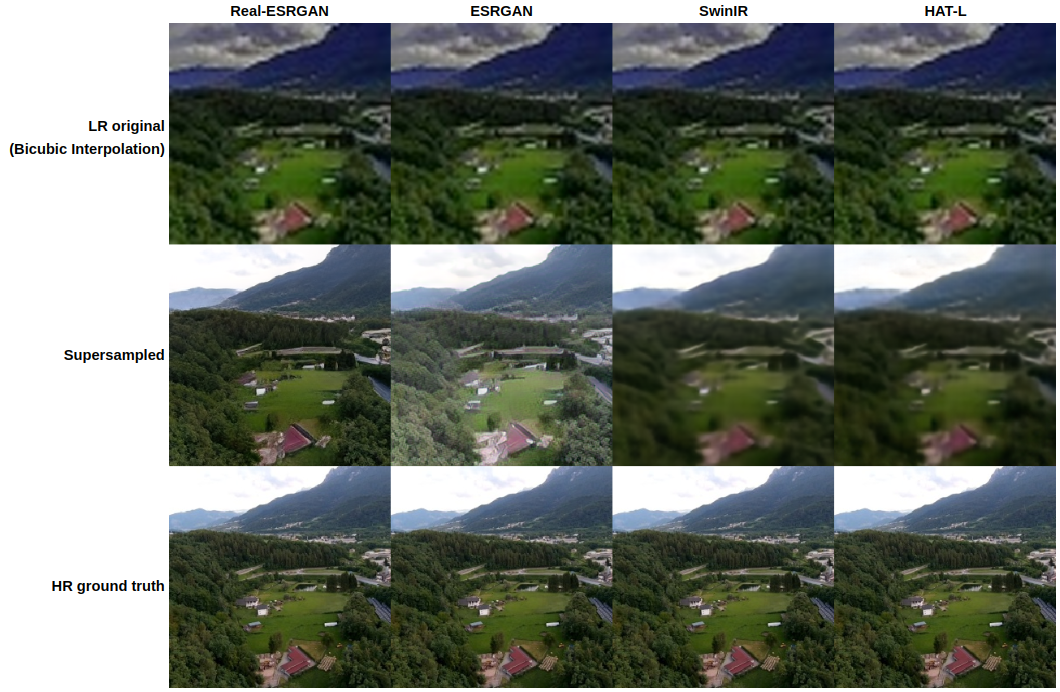
\includegraphics[scale=0.3]{figures/allegati/sbs_1.png}
  \label{img:sbs1}
\end{figure}
\begin{figure}[H]
  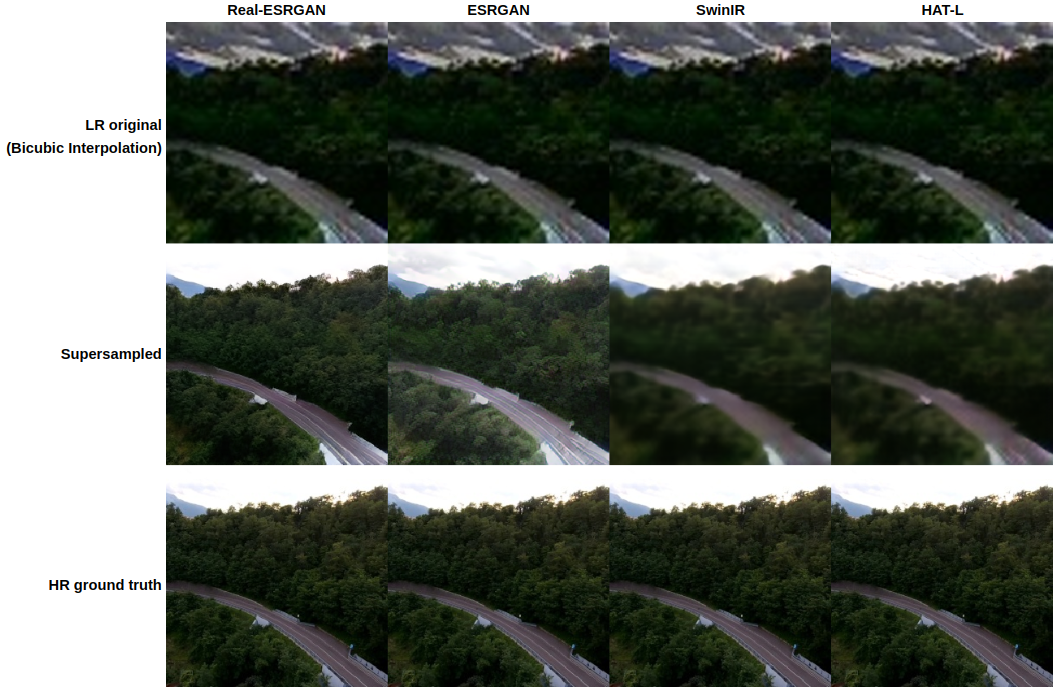
\includegraphics[scale=0.3]{figures/allegati/sbs_2.png}
  \label{img:sbs2}
\end{figure}
\begin{figure}[H]
  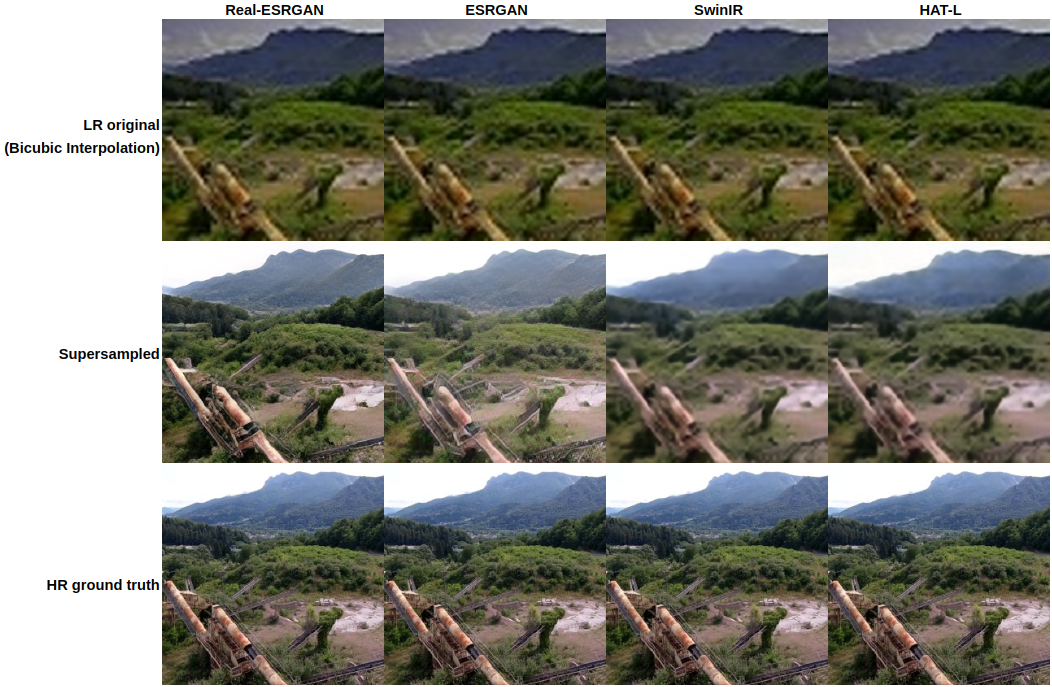
\includegraphics[scale=0.3]{figures/allegati/sbs_3.png}
  \label{img:sbs3}
\end{figure}

\section{Supersampled images}
All the images are, from top to bottom, orignal LR resized to 4 times its orignal size with bicubic interpolation, generated image by supersampling with scale 4, HR ground truth.
\subsection{Real-ESRGAN}

\begin{figure}[H]
  \centering
  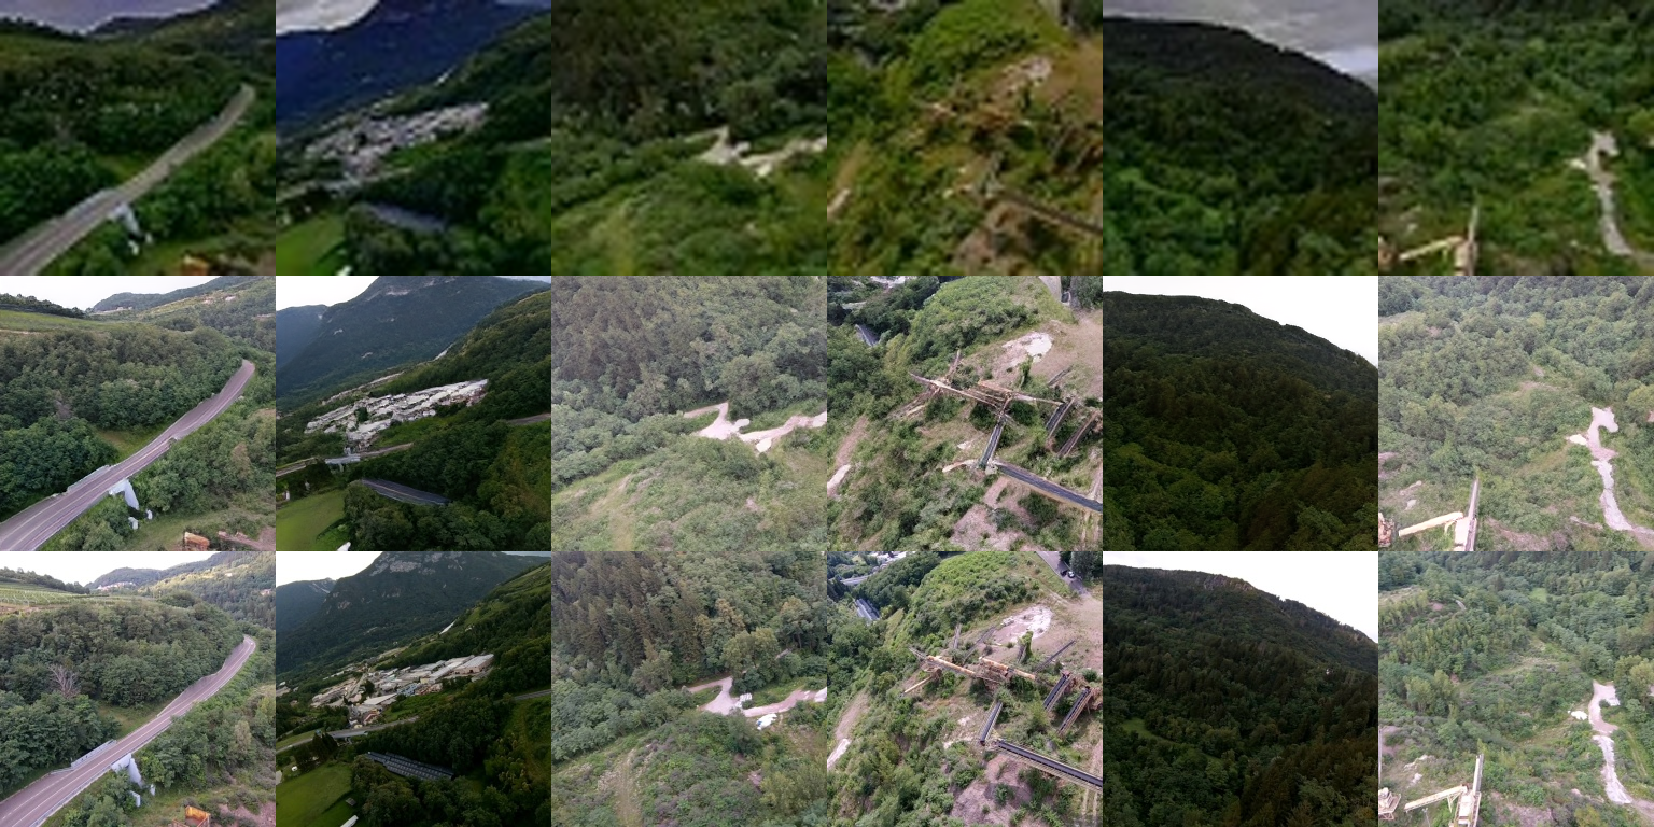
\includegraphics[scale=0.37]{figures/allegati/realesrgan64.png}
  \caption{From the 64 to 256 dataset.}
  \label{img:realesrgan_training}
\end{figure}

\begin{figure}[H]
  \centering
  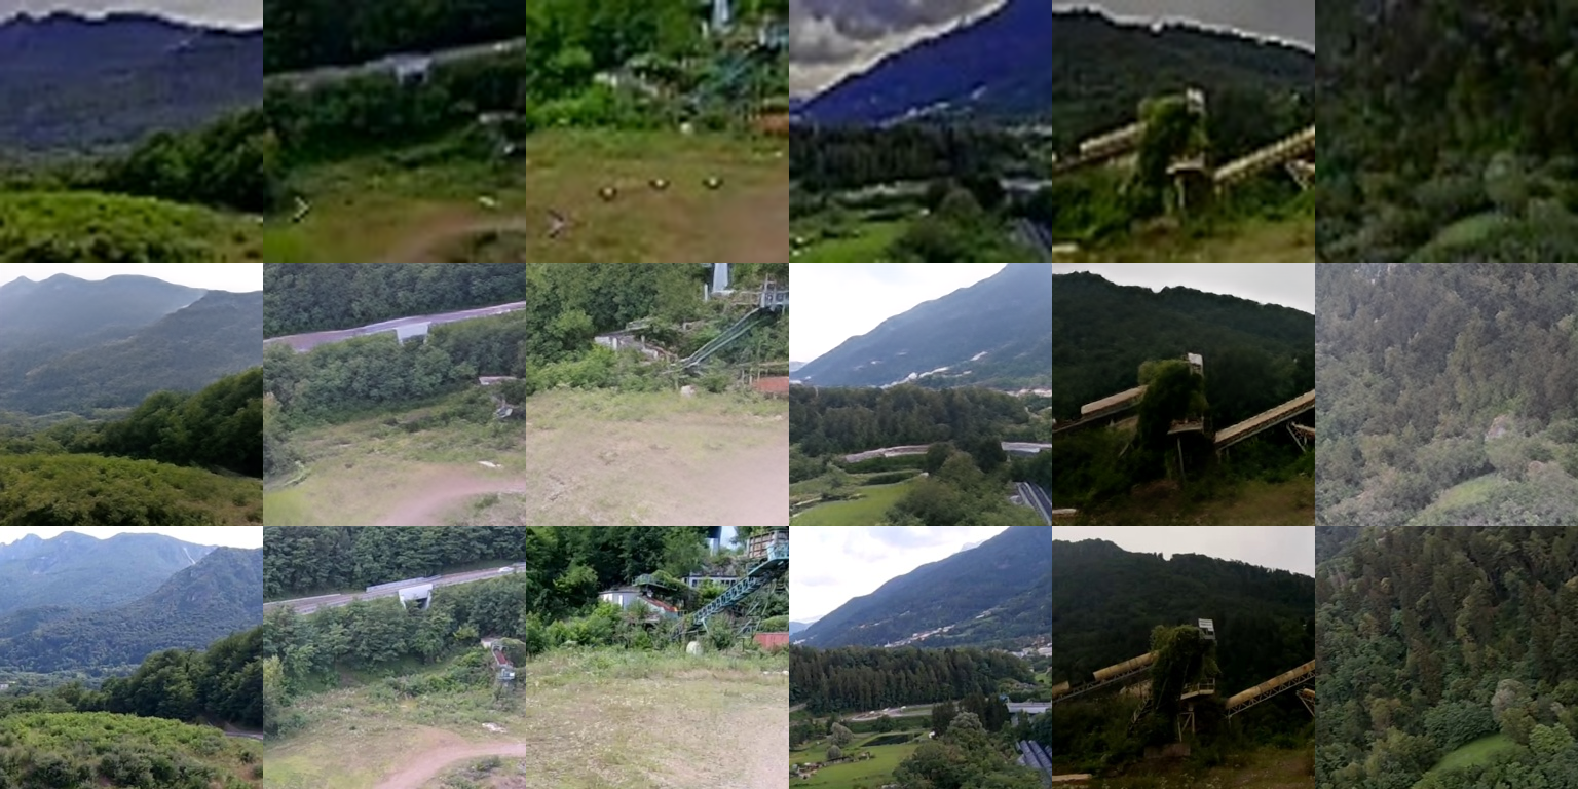
\includegraphics[scale=0.37]{figures/allegati/realesrgan64p.png}
  \caption{From the 64 to 256 patches dataset.}
  \label{img:realesrgan_training}
\end{figure}

\begin{figure}[H]
  \centering
  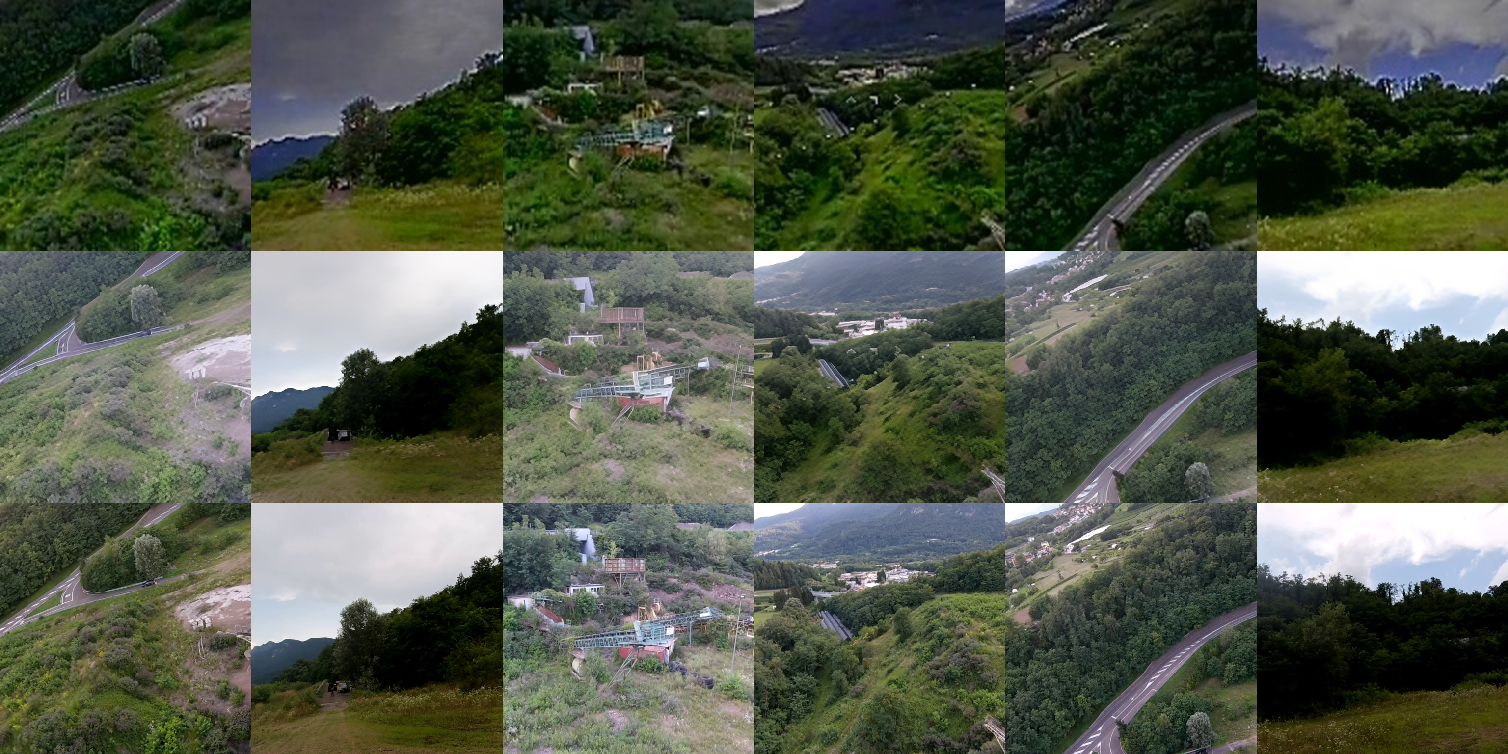
\includegraphics[scale=0.39]{figures/allegati/realesrgan128.png}
  \caption{From the 128 to 512 dataset.}
  \label{img:realesrgan_training}
\end{figure}
